% \preto\tabular{\setcounter{reqid}{0}}
\newcounter{reqid}
\newcounter{caseid}
\newcommand\req{%
  \stepcounter{reqid}%
  R-\padzeroes[3]{\decimal{reqid}}
}
\newcommand\reqcase{%
  \stepcounter{caseid}%
  C-\padzeroes[3]{\decimal{caseid}}
}
\newcolumntype{L}{>{\centering\arraybackslash}m{2.5cm}}

\chapter{An\'alisis de requisitos, dise\~no e implementaci\'on}\label{requisitos}

\section{Requisitos de información}
\subsection{Usuarios}
\begin{itemize}
  \item Nombre de usuario
  \item Contraseña
\end{itemize}
\subsection{Sala de espera}
\begin{itemize}
  \item Usuarios en la sala
  \item Reglas de la casa
  \item Baraja escogida
\end{itemize}
\subsection{Cartas}
\begin{itemize}
  \item Color
  \item Símbolo
\end{itemize}
\subsection{Partida}
\begin{itemize}
  \item Jugador del turno actual
  \item Cartas en la baraja
  \item Cartas en la pila de descartes
  \item Jugadores asociados
  \item Orientación de turnos
\end{itemize}
\subsection{Jugadores}
\begin{itemize}
  \item Cartas en mano
\end{itemize}

\section{Tipos de usuario}
En la aplicación, solo habrá una distinción de los usuarios en la sala de espera.
En los demás aspectos, todos los usuarios tendrán los mismos permisos.

En la sala de espera, habrá 2 roles distintos:
\begin{description}
  \item[Jugador normal:] Usuario que únicamente puede marcar si está listo o no y mandar mensajes 
    en el chat.
  \item[Huésped:] Usuario que ha creado la sala de espera y puede modificar
    las reglas y mazo a usar en el juego.
\end{description}

\section{Historias de usuario}
\subsection{Autenticación de usuario}

\subsubsection{Registro de usuario}

Como usuario sin autenticar, quiero poder registrarme en el sistema con un usuario y contraseña para poder acceder al juego. 

\subparagraph{Caso positivo} % (fold)

El usuario rellena un formulario en el que pone de nombre de usuario Pepito123 y contraseña MeGustanLosJabalies, tras hacer click en el botón de enviar, se mandarán los datos al servidor, que creará el usuario correspondiente e iniciará la sesión del usuario. 

\subsubsection{Inicio de sesión de usuario}

Como usuario sin autenticar, quiero poder usar mi usuario y contraseña para acceder a mi cuenta dentro de la aplicación y así acceder al juego. 

\subparagraph{Caso positivo}

El usuario sin autenticar, que se ha registrado anteriormente como Pepito123 y ha puesto de contraseña MeGustanLosJabalies, rellena un formulario en el que provee dichos datos, y tras darle al botón de enviar el sistema comprobará que la contraseña es la correcta para ese usuario y le dejará iniciar sesión. 

\subparagraph{Caso negativo 1}

Un usuario sin autenticar, que no se ha registrado anteriormente, provee en el formulario de inicio de sesión datos de usuario y contraseña que no existen en el sistema. El formulario se vuelve a mostrar, mostrando un mensaje de que los datos dados son incorrectos. 

\subparagraph{Caso negativo 2}

El usuario sin autenticar provee en el formulario un nombre correcto de usuario, pero pone una contraseña incorrecta. El formulario se vuelve a mostrar, con un mensaje mostrando que los datos introducidos son incorrectos. 

\subsection{Sala de espera}

\subsubsection{Crear una sala de espera }

Como usuario autenticado, quiero poder crear una sala de juego, para esperar a que otras personas entren antes de empezar el juego. 

\subparagraph{Caso positivo}

El usuario, tras autenticarse, hace click en un botón de “crear partida” y se le llevará directamente a una nueva sala de espera 

\subparagraph{Caso negativo }

El usuario, sin autenticar, hace click en un botón de “crear partida”, pero como no está autenticado, se le llevará a la página de autenticarse, indicando que debe iniciar sesión para crear la partida. 

\subsubsection{Unirse a una sala de espera }

Como usuario, quiero poder acceder a una sala de juego ya existente, para poder participar en el juego con los jugadores de dicha sala. 

\subparagraph{Caso positivo 1}

El usuario, tras autenticarse, hace click en un botón de “unirse a partida”, donde se le presentará un formulario donde podrá proveer el código de la partida, y una vez introduzca un código válido y le dé al botón de enviar, se le llevará a la sala de espera correspondiente 

\subparagraph{Caso positivo 2}

El usuario, tras autenticarse, usa un enlace que le ha dado el huésped de la partida que va a jugar, y al abrirlo se meterá automáticamente en la sala de espera 

\subparagraph{Caso negativo 1}

El usuario, sin autenticarse, hace click en un botón de “unirse a partida” y se le llevará a la página de autenticación, indicando que tiene que iniciar sesión. 

\subparagraph{Caso negativo 2}
El usuario, sin autenticarse, usa un enlace que le ha dado el huésped de la partida, y al abrirlo se le redirigirá a la página de autenticarse, indicando que tiene que iniciar sesión. 

\subparagraph{Caso negativo 3}
El usuario, tras autenticarse, pone en el formulario de unirse a una partida un código de una partida que no existe. Al darle click al botón de enviar, se le indicará que no existe esa partida y se le mostrará de nuevo el formulario. 

\subparagraph{Caso negativo 4}
El usuario, tras autenticarse, pone en el formulario de unirse a una partida un código de una partida que está en curso. Al darle click al botón de enviar, se le indicará que la partida está en curso y se le mostrará de nuevo el formulario. 

\subsubsection{Marcar estado de “listo” en sala de espera}

Como usuario, quiero poder marcar que estoy listo para empezar la partida, para así comunicar al huésped de la sala que puede comenzar la partida sin miedo a que yo me la pierda. 

\subparagraph{Caso positivo}

Un jugador no huésped le da a un botón de “Listo”, y para todos los demás jugadores y el huésped se les mostrará dicho estado. 

\subsubsection{Iniciar partida en sala de espera}

Como usuario y huésped en una sala de espera, quiero empezar la partida una vez haya observado que se han unido a la sala todas las personas que esperaba y que estén listas, para poder jugar con todas ellas. 

\subparagraph{Caso positivo}

El jugador huésped de una sala de espera, tras observar que todos los demás jugadores están listos para empezar la partida, hace click en un botón de Empezar Partida, y, tras ello, todos los jugadores serán redirigidos a la partida. 

\subsubsection{Configurar Reglas de la Casa}

Como usuario, al crear una sala de espera quiero poder escoger las reglas especiales a aplicar, para acomodar las preferencias mías y de mis compañeros al jugar. 

\subparagraph{Caso positivo}

El jugador huésped de una sala de espera hace click en la casilla de la regla de la intercepción para activarla durante la partida. 

Como jugador dentro de una partida, quiero poder especificar que digo “Uno” cuando me quedo con 1 carta en mano para poder cumplir con las normas del juego. 

\subsubsection{Configurar mazo}

Como usuario, quiero poder configurar el mazo de cartas de la partida antes de comenzarla,
para customizar la experiencia del juego a mi gusto.

\subparagraph{Caso positivo}

El jugador huésped de una sala de espera hace click en una casilla correspondiente al
mazo que se quiera escoger. Cuando se inicie el juego, este usará la baraja seleccionada.

\subsection{Juego}

Como usuario, quiero poder jugar al juego de cartas con otros jugadores, para poder
socializar y divertirme.

\subsection{Chat}

Como usuario, quiero poder comunicarme con otros jugadores en la partida y en la sala de espera, para así
poder socializar durante esta y coordinarme con los demás jugadores para coordinarnos en
las customizaciones que queramos aplicar.

\subparagraph{Caso positivo}

El jugador dentro de una sala de espera rellena un campo de texto para el chat y le da al botón de enviar.
Los demás jugadores en la sala reciben el mensaje en la sección del chat.


\subparagraph{Caso positivo}

El jugador dentro de un juego rellena un campo de texto para el chat y le da al botón de enviar.
Los demás jugadores en la sala reciben el mensaje en la sección del chat.

\section{Matriz de trazabilidad de requisitos} % (fold)

\begin{tabular}{|L|L|L|L|}

\hline
Requisitos & Entorno de ocio & Socialización & Experiencia customizable \\
\hline

Autenticación de usuario & & & \\
\hline
Inicio de sesión & & & \\
\hline
Sala de espera & &\checkmark & \checkmark \\
\hline
Configuración reglas de la casa & & &\checkmark \\
\hline
Configuración mazos de cartas & & & \checkmark  \\
\hline
Chat & \checkmark & \checkmark & \\
\hline
Juego & \checkmark & \checkmark & \\
\hline

\end{tabular}

% section  (end)

\section{Dise\~no e implementaci\'on}

\subsection{Arquitectura del sistema}

Se realizará una arquitectura por capas compuesta por:

\begin{itemize}
  \item Capa de presentación
  \item Capa de servidor
  \item Capa de datos
\end{itemize}

\subsubsection{Capa de datos}
Se realizará usando MongoDB para una base de datos NoSQL,
debido a que puede acomodar más fácilmente la estructura del juego,
comparado con una base de datos relacional.

Esto también resulta en mayor rendimiento, ya que se evitan algunas operaciones de unión de tablas.

\paragraph{Esquema de la base de datos}

\begin{center}
  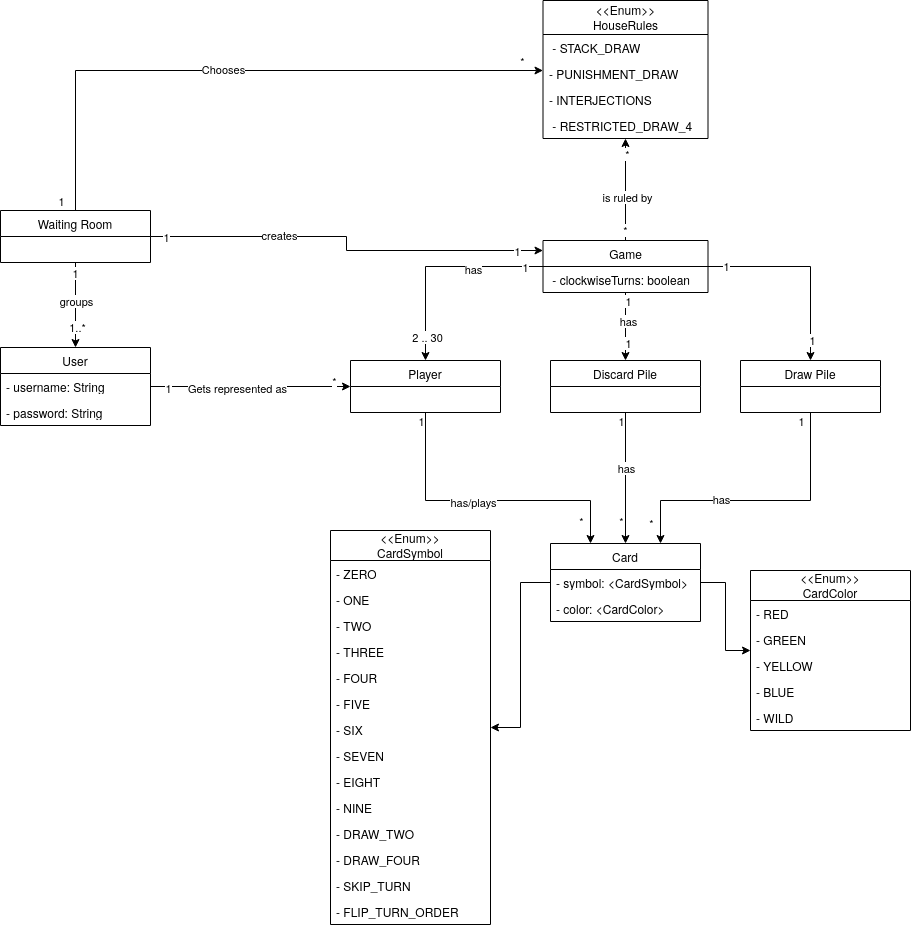
\includegraphics[width=1\textwidth]{img/BD_drawio.png}
  \captionof{figure}{Representación UML de la base de datos} \label{fig:dbschema}
\end{center}

\subsubsection{Capa de servidor}
Se creará en lenguaje JavaScript debido a la familiaridad con el mismo, aunque se añadirá al mismo tiempo TypeScript. 

Al mismo tiempo, se incorporará Bun,
ya que provee mayor rendimiento y soporte nativo para TypeScript,
así como otras funcionalidades como la ejecución de tests. 

Como framework, se hará uso de Elysia como framework de Backend, ya que está intencionado para su uso con Bun
y es soportado por varias plataformas de despliegue. 

\paragraph{Documentación de la API:}

La API del servidor se documentará con las especificaciones de OpenAPI para las rutas normales.
Las rutas de WebSocket se documentarán manualmente.

\subparagraph{Rutas de la API REST:}

\begin{itemize}
  \item /user
    \begin{description}
      \item[POST:] Registra un nuevo usuario
        \begin{description}
          \item[username:] Nombre de usuario
          \item[password:] Contraseña
        \end{description}
    \end{description}
    \begin{itemize}
      \item /login
        \begin{description}
          \item[POST:] Inicia sesión del usuario
            \begin{description}
              \item[username:] Nombre de usuario
              \item[password:] Contraseña
            \end{description}
        \end{description}
    \end{itemize}
  \item /room
      \begin{description}
      \item[POST:] Crea una sala de espera nueva asociada al usuario actual
      \end{description}
\end{itemize}
\subparagraph{Rutas de la API WebSockets:}
% TODO: Add Websocket API routes
\begin{itemize}
  \item Test
\end{itemize}

\subsubsection{Capa de presentación}

Se realizará también con JavaScript y Bun, por razones similares a las de la capa de servidor. 

Se usará el framework de React debido a su gran cantidad de documentación y popularidad,
así como por la experiencia previa que se ha tenido con dicho framework. 

Adicionalmente, otras tecnologías que se usarán en este apartado son Vite para
utilidades de desarrollo, y para el estilado se usará Tailwind, así como Shadcn.ui.

Tailwind se ha escogido debido a que simplifica el proceso de diseño de estilos,
y gracias a los componentes de React se pueden abstraer y reutilizar fácilmente
a través de toda la aplicación. 

Shacn.ui, por otro lado, se ha escogido debido a que proporciona componentes
que se instalan directamente en el código en vez de depender de una librería externa.
Esto logra que los componentes sean muy customizables y se puedan usar como punto de partida,
ya que proveen los detalles más difíciles como la accesibilidad ya integrados.

\paragraph{Mockups}

\begin{center}
  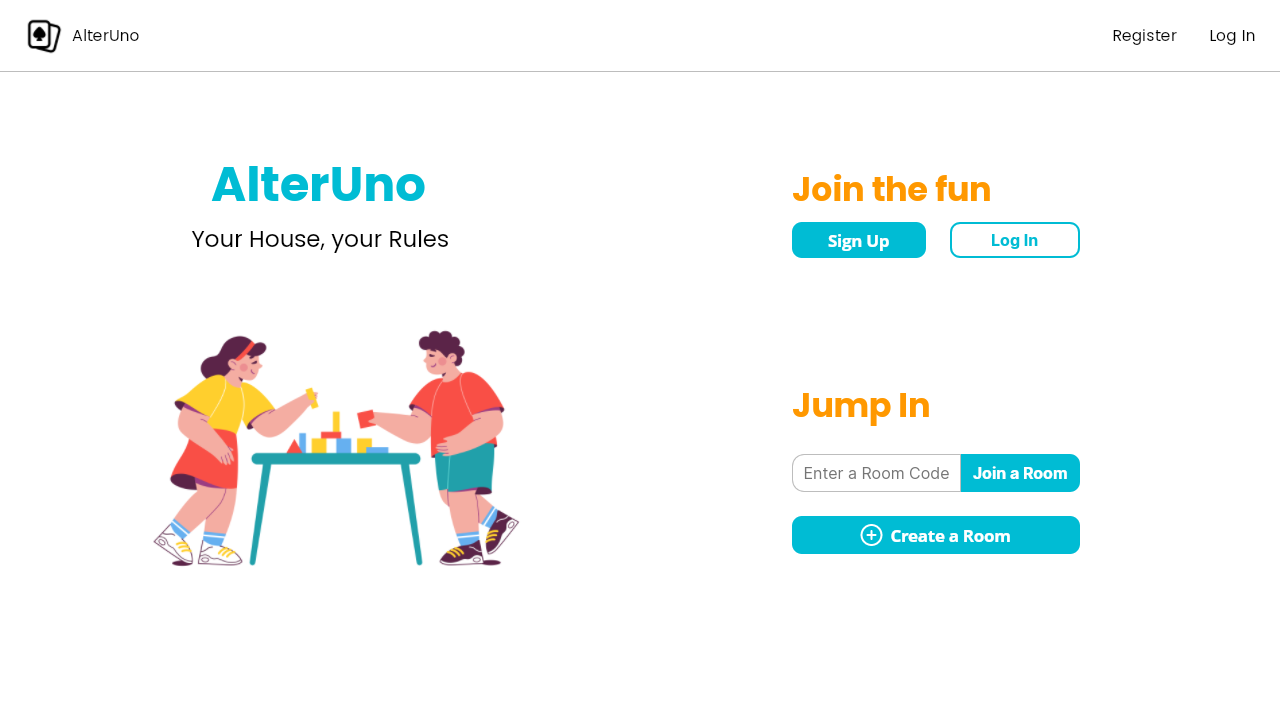
\includegraphics[width=1\textwidth]{img/Mockup Main Page}
  \captionof{figure}{Mockup de la pantalla de inicio} \label{fig:mainmockup}
\end{center}

\begin{center}
  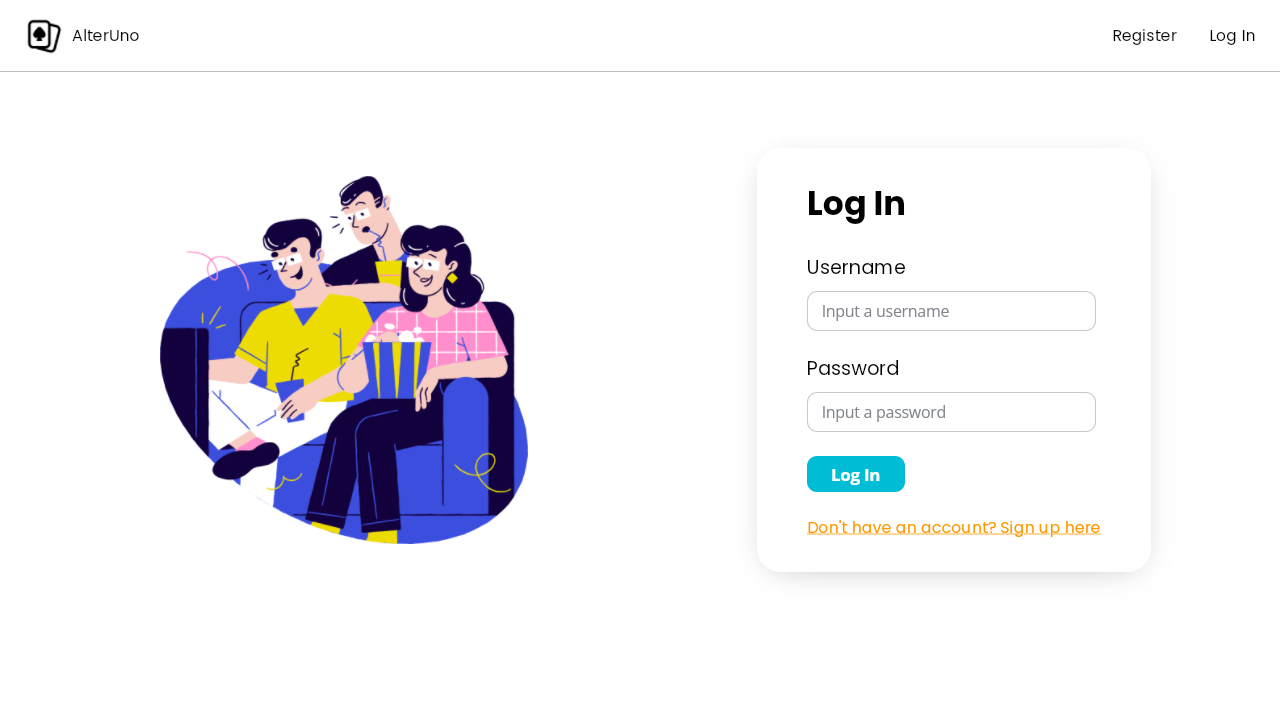
\includegraphics[width=1\textwidth]{img/Mockup Log In}
  \captionof{figure}{Mockup de la pantalla de inicio de sesión} \label{fig:loginmockup}
\end{center}

\begin{center}
  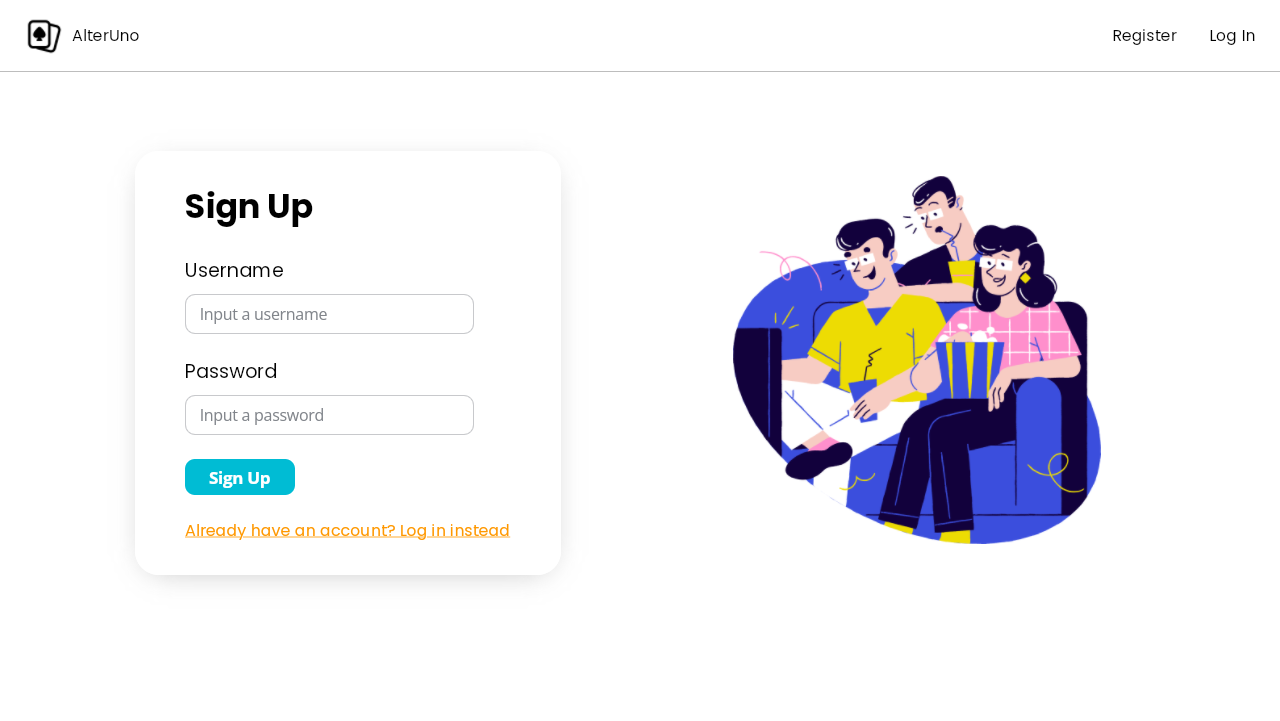
\includegraphics[width=1\textwidth]{img/Mockup Sign Up}
  \captionof{figure}{Mockup de la pantalla de registro} \label{fig:signupmockup}
\end{center}


\begin{center}
  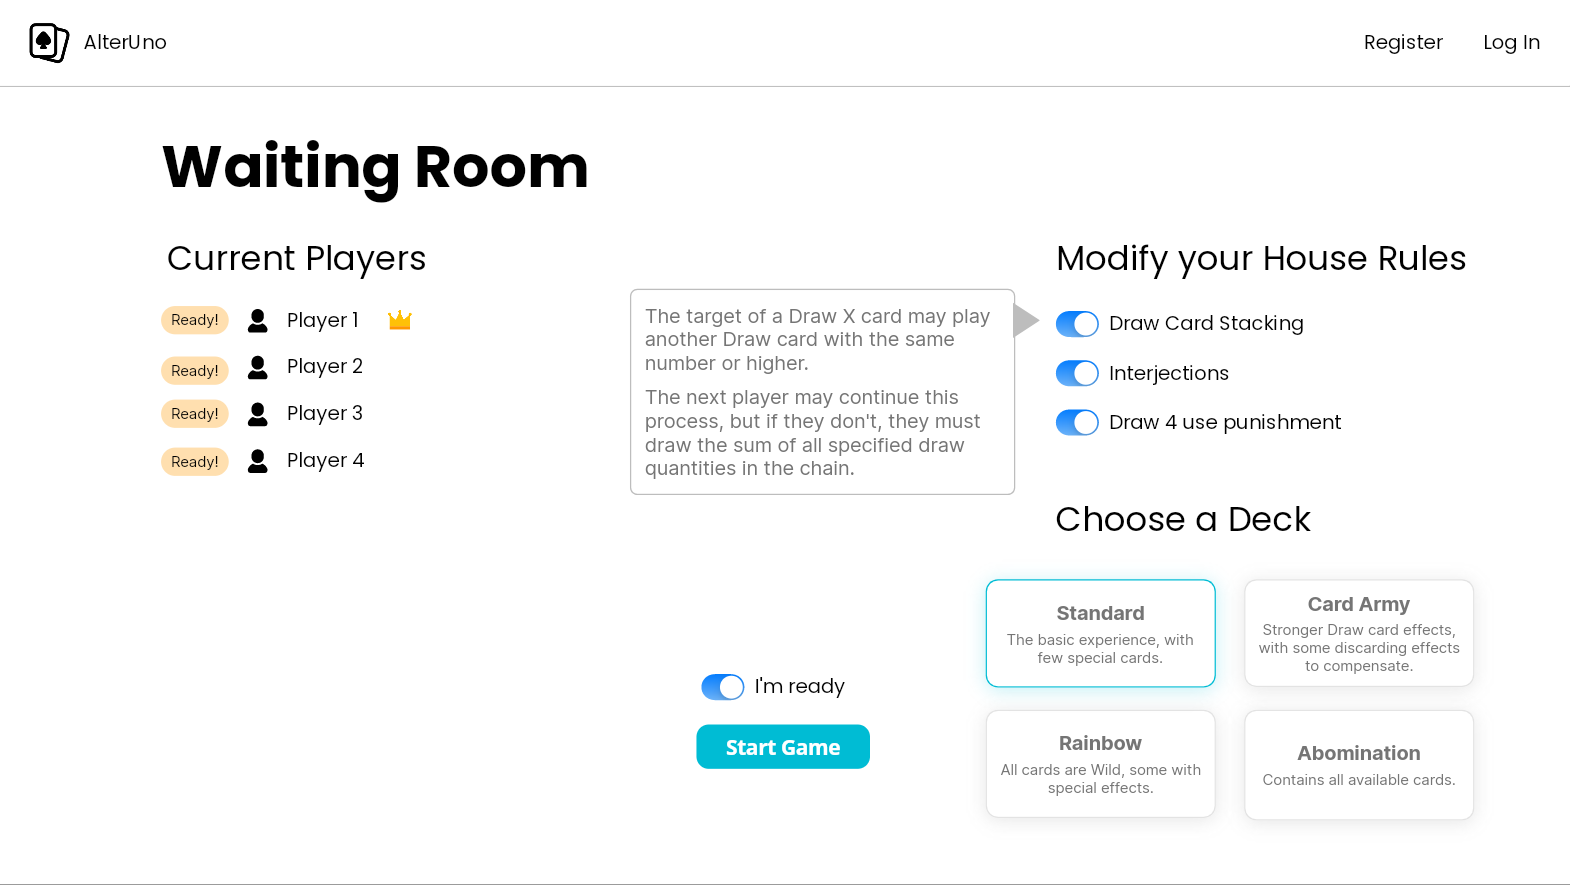
\includegraphics[width=1\textwidth]{img/Mockup Waiting Room}
  \captionof{figure}{Mockup de la pantalla de sala de espera} \label{fig:waitingroommockup}
\end{center}

\begin{center}
  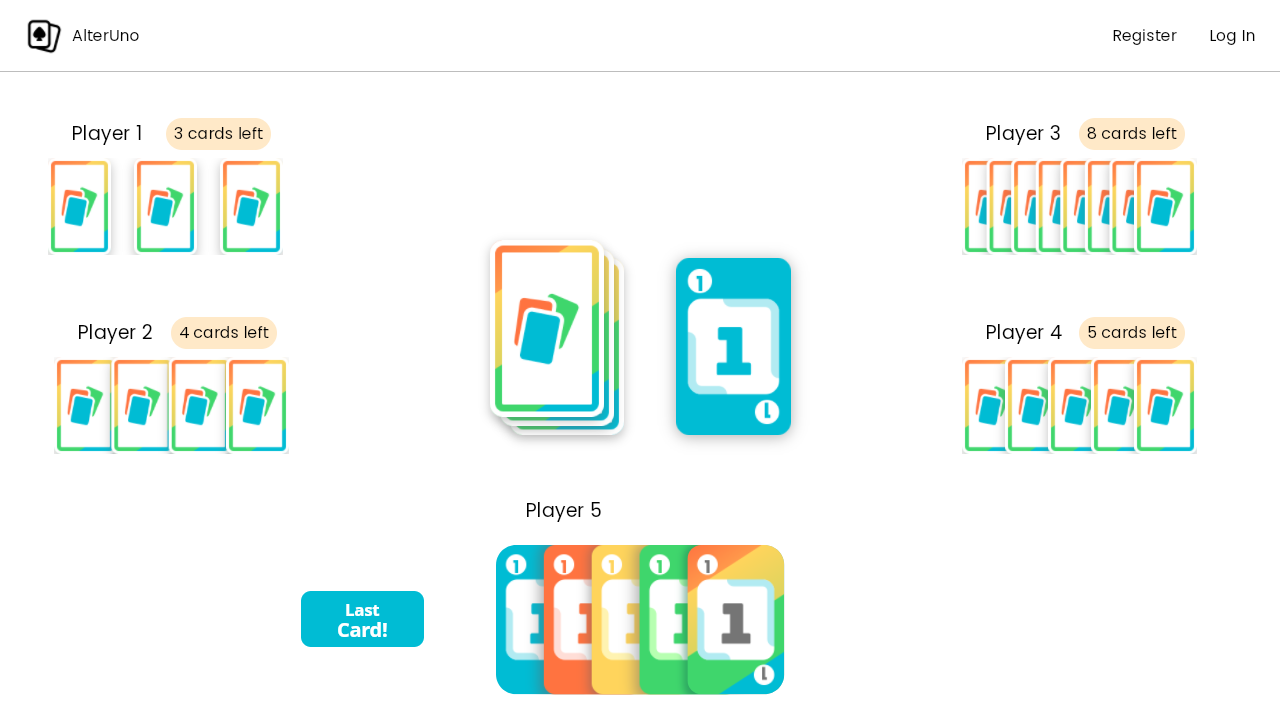
\includegraphics[width=1\textwidth]{img/Mockup Game}
  \captionof{figure}{Mockup de la pantalla del juego} \label{fig:gamemockup}
\end{center}


